After having agreed on a set of project requirements, deadlines and objectives in collaboration with the students from Singapore, we needed to plan how to meet those objectives within the project deadline. As such we began planning what work needed to be done and what activities we expected to do in the project.
During the planning process and the associated discussion it became clear to us, that in order to make a realistic plan for the project, we needed a more in-depth understanding of the work and activities lying ahead. In order to see “the big picture”, we decided to use an approach from Cadle\&Yeates \cite{caye} known as a \emph{work breakdown structure}. The work breakdown structure is organized in a hierarchical tree structure, where each new level in the tree is created by dividing a task into subtasks as shown on figure \ref{fig:breakdown}.

\begin{figure}[hbtp]
	\label{fig:breakdown}
	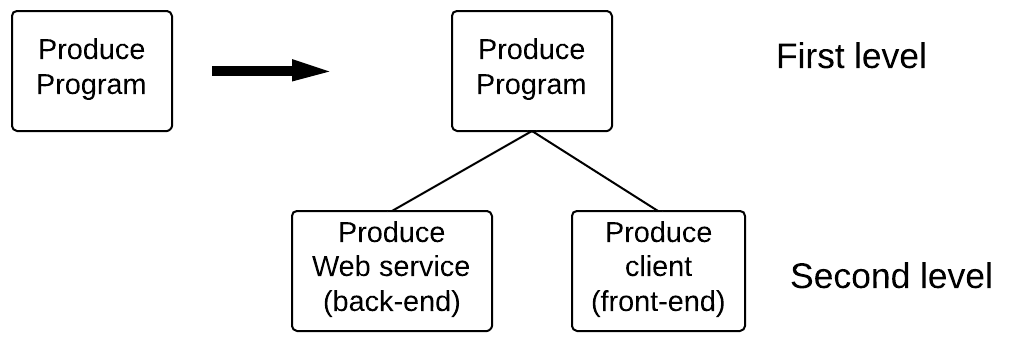
\includegraphics[scale=0.5]{./Empiri/Planning/img/wbslevels.png}
	\caption{Example work breakdown structure} 
\end{figure}
The division of tasks into smaller components is an iterative process, which stops when the resulting tasks are small enough to be considered a suitable assignment for one man or, more subjectively, when it simply does not make sense to divide it any further.
The use of a work breakdown structure did require several long discussions among the team members regarding the identification of the work. Our use of the work breakdown structure was especially prone to discussion as the problem domain was rather new for us and it was difficult to conclude on what needed to be done, since we had no experience to draw on.
Our complete work breakdown structure can be found in appendix \textbf{insert reference here}.

%\textbf{Til analyse-tabere:
%Konklusionen som jeg prøver at lægge lidt op til er at vi skulle have brugt product breakdown structure i stedet. Se side 119 i bogen.
%Et product breakdown structure sørger for at fokus holdes på HVAD der skal opnås, fremfor HVORDAN det skal opnås og det er specielt velegnet til nye arbejdsområder, hvor det kan være svært at se hvilket arbejde der er nødvendigt, men nemmere at identificere de produkter det skal ende ud i.}
